% Figure 6: Multi-Model Pareto Frontier — K=5 and K=10
% Include from the main paper via % Figure 6: Multi-Model Pareto Frontier — K=5 and K=10
% Include from the main paper via % Figure 6: Multi-Model Pareto Frontier — K=5 and K=10
% Include from the main paper via % Figure 6: Multi-Model Pareto Frontier — K=5 and K=10
% Include from the main paper via \input{../experiments/06_figure/figure_6_caption}

\begin{figure*}[t]
\centering
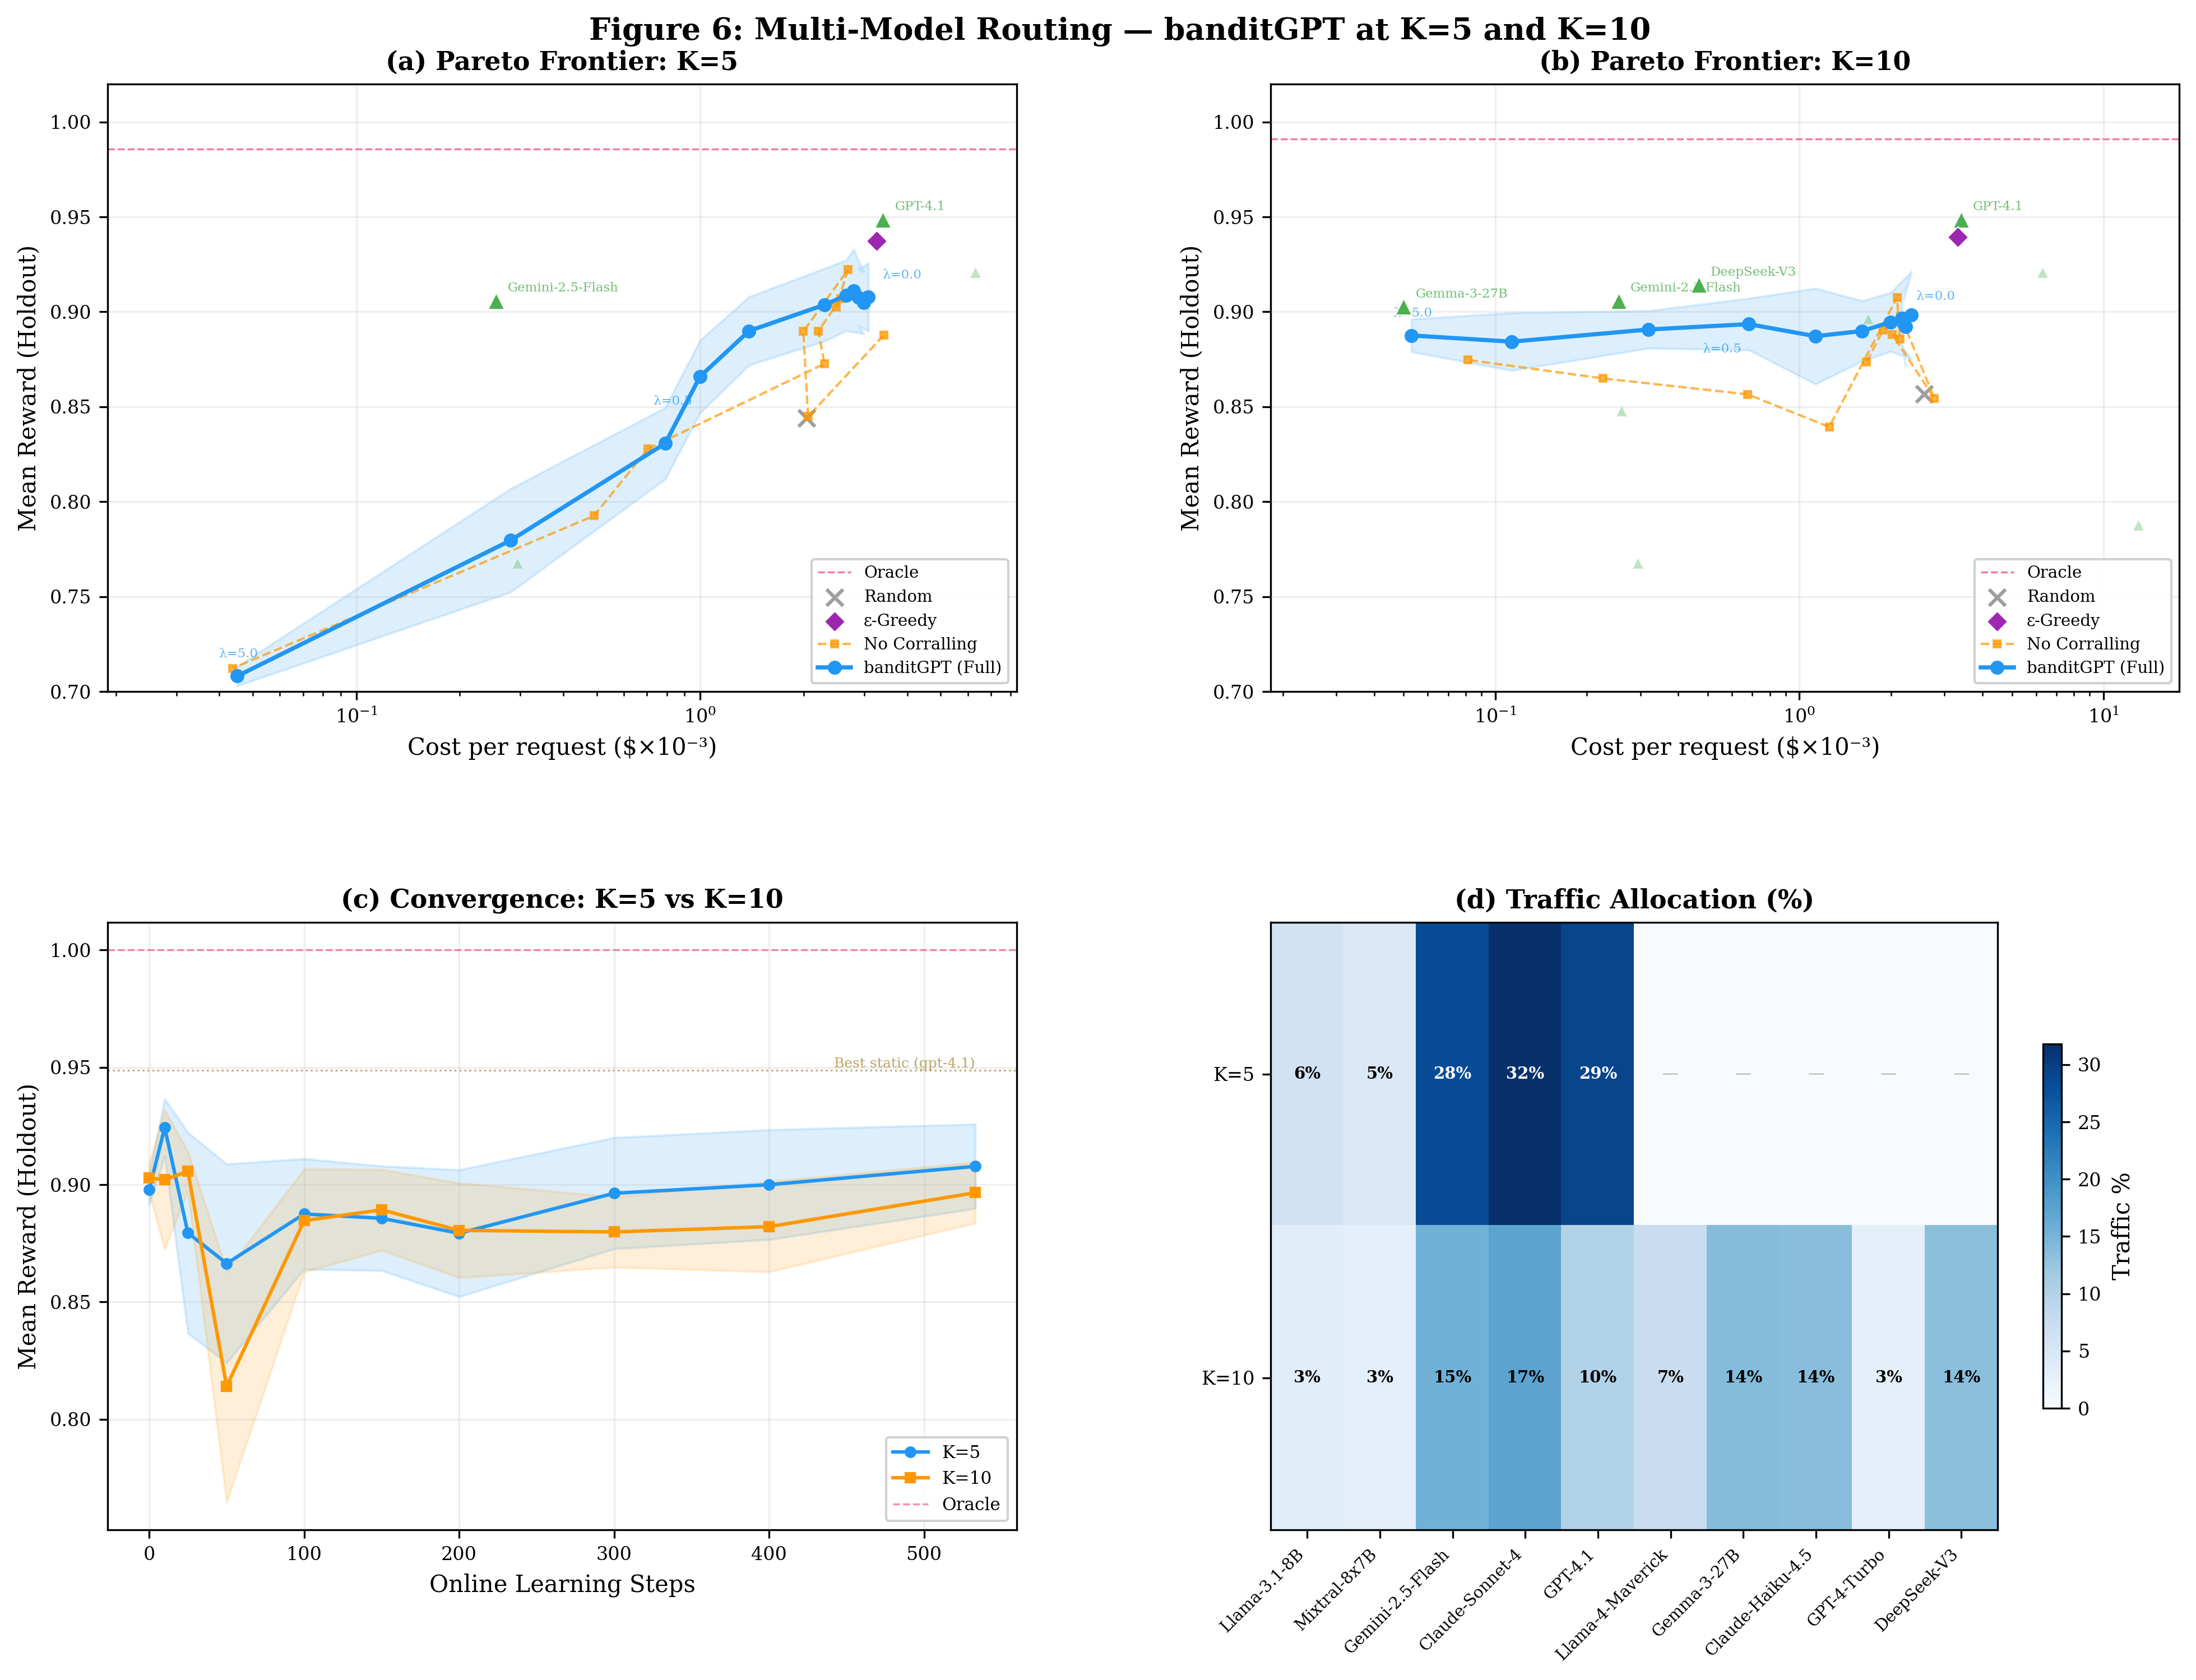
\includegraphics[width=0.95\textwidth]{../experiments/06_figure/results/figure6_multimodel_pareto.png}
\caption{\textbf{Multi-model routing at $K{=}5$ and $K{=}10$: cost--quality Pareto frontiers, convergence, and traffic allocation.} Reward is mean judge agreement across a 3--4 member LLM panel (continuous in $[0,1]$).
\textbf{(a,b)}~Pareto frontiers sweeping cost penalty $\lambda \in [0, 5]$ ($n{=}20$ seeds per point; log-scaled cost axis). Labelled green triangles mark Pareto-efficient static baselines; faded triangles show dominated models. The blue curve traces banditGPT's operating envelope. At peak quality ($\lambda{=}0.02$), banditGPT achieves 0.911 (K{=}5) and 0.898 (K{=}10). At $\lambda{=}5$ (cost-minimising), it routes nearly all traffic to the cheapest model while maintaining 0.708 (K{=}5) and 0.888 (K{=}10) quality. The orange dashed line (no Corralling) shows the ablated system without the meta-learner.
\textbf{(c)}~Convergence from warmup priors: both portfolios start at ${\sim}0.90$ reward (step~0, no online learning), demonstrating that the 43-model warmup priors provide effective cold-start quality across portfolio sizes. K{=}5 improves to 0.911 by step 533; K{=}10 remains stable at ${\sim}0.88{-}0.90$.
\textbf{(d)}~Traffic allocation on the holdout set ($\lambda{=}0$). At K{=}5, the router concentrates on three high-quality models (Claude-Sonnet: 32\%, GPT-4.1: 29\%, Gemini-Flash: 28\%) while using cheaper models sparingly (${\leq}6\%$). At K{=}10, traffic distributes across all models (3--17\% each), reflecting contextual per-prompt routing rather than static model selection.
Evaluation protocol: 533 online-learning prompts (three-way split, disjoint from prior training), frozen holdout of 750 prompts (identical to Section~\ref{sec:pareto}).}
\label{fig:multimodel_pareto}
\end{figure*}


\begin{figure*}[t]
\centering
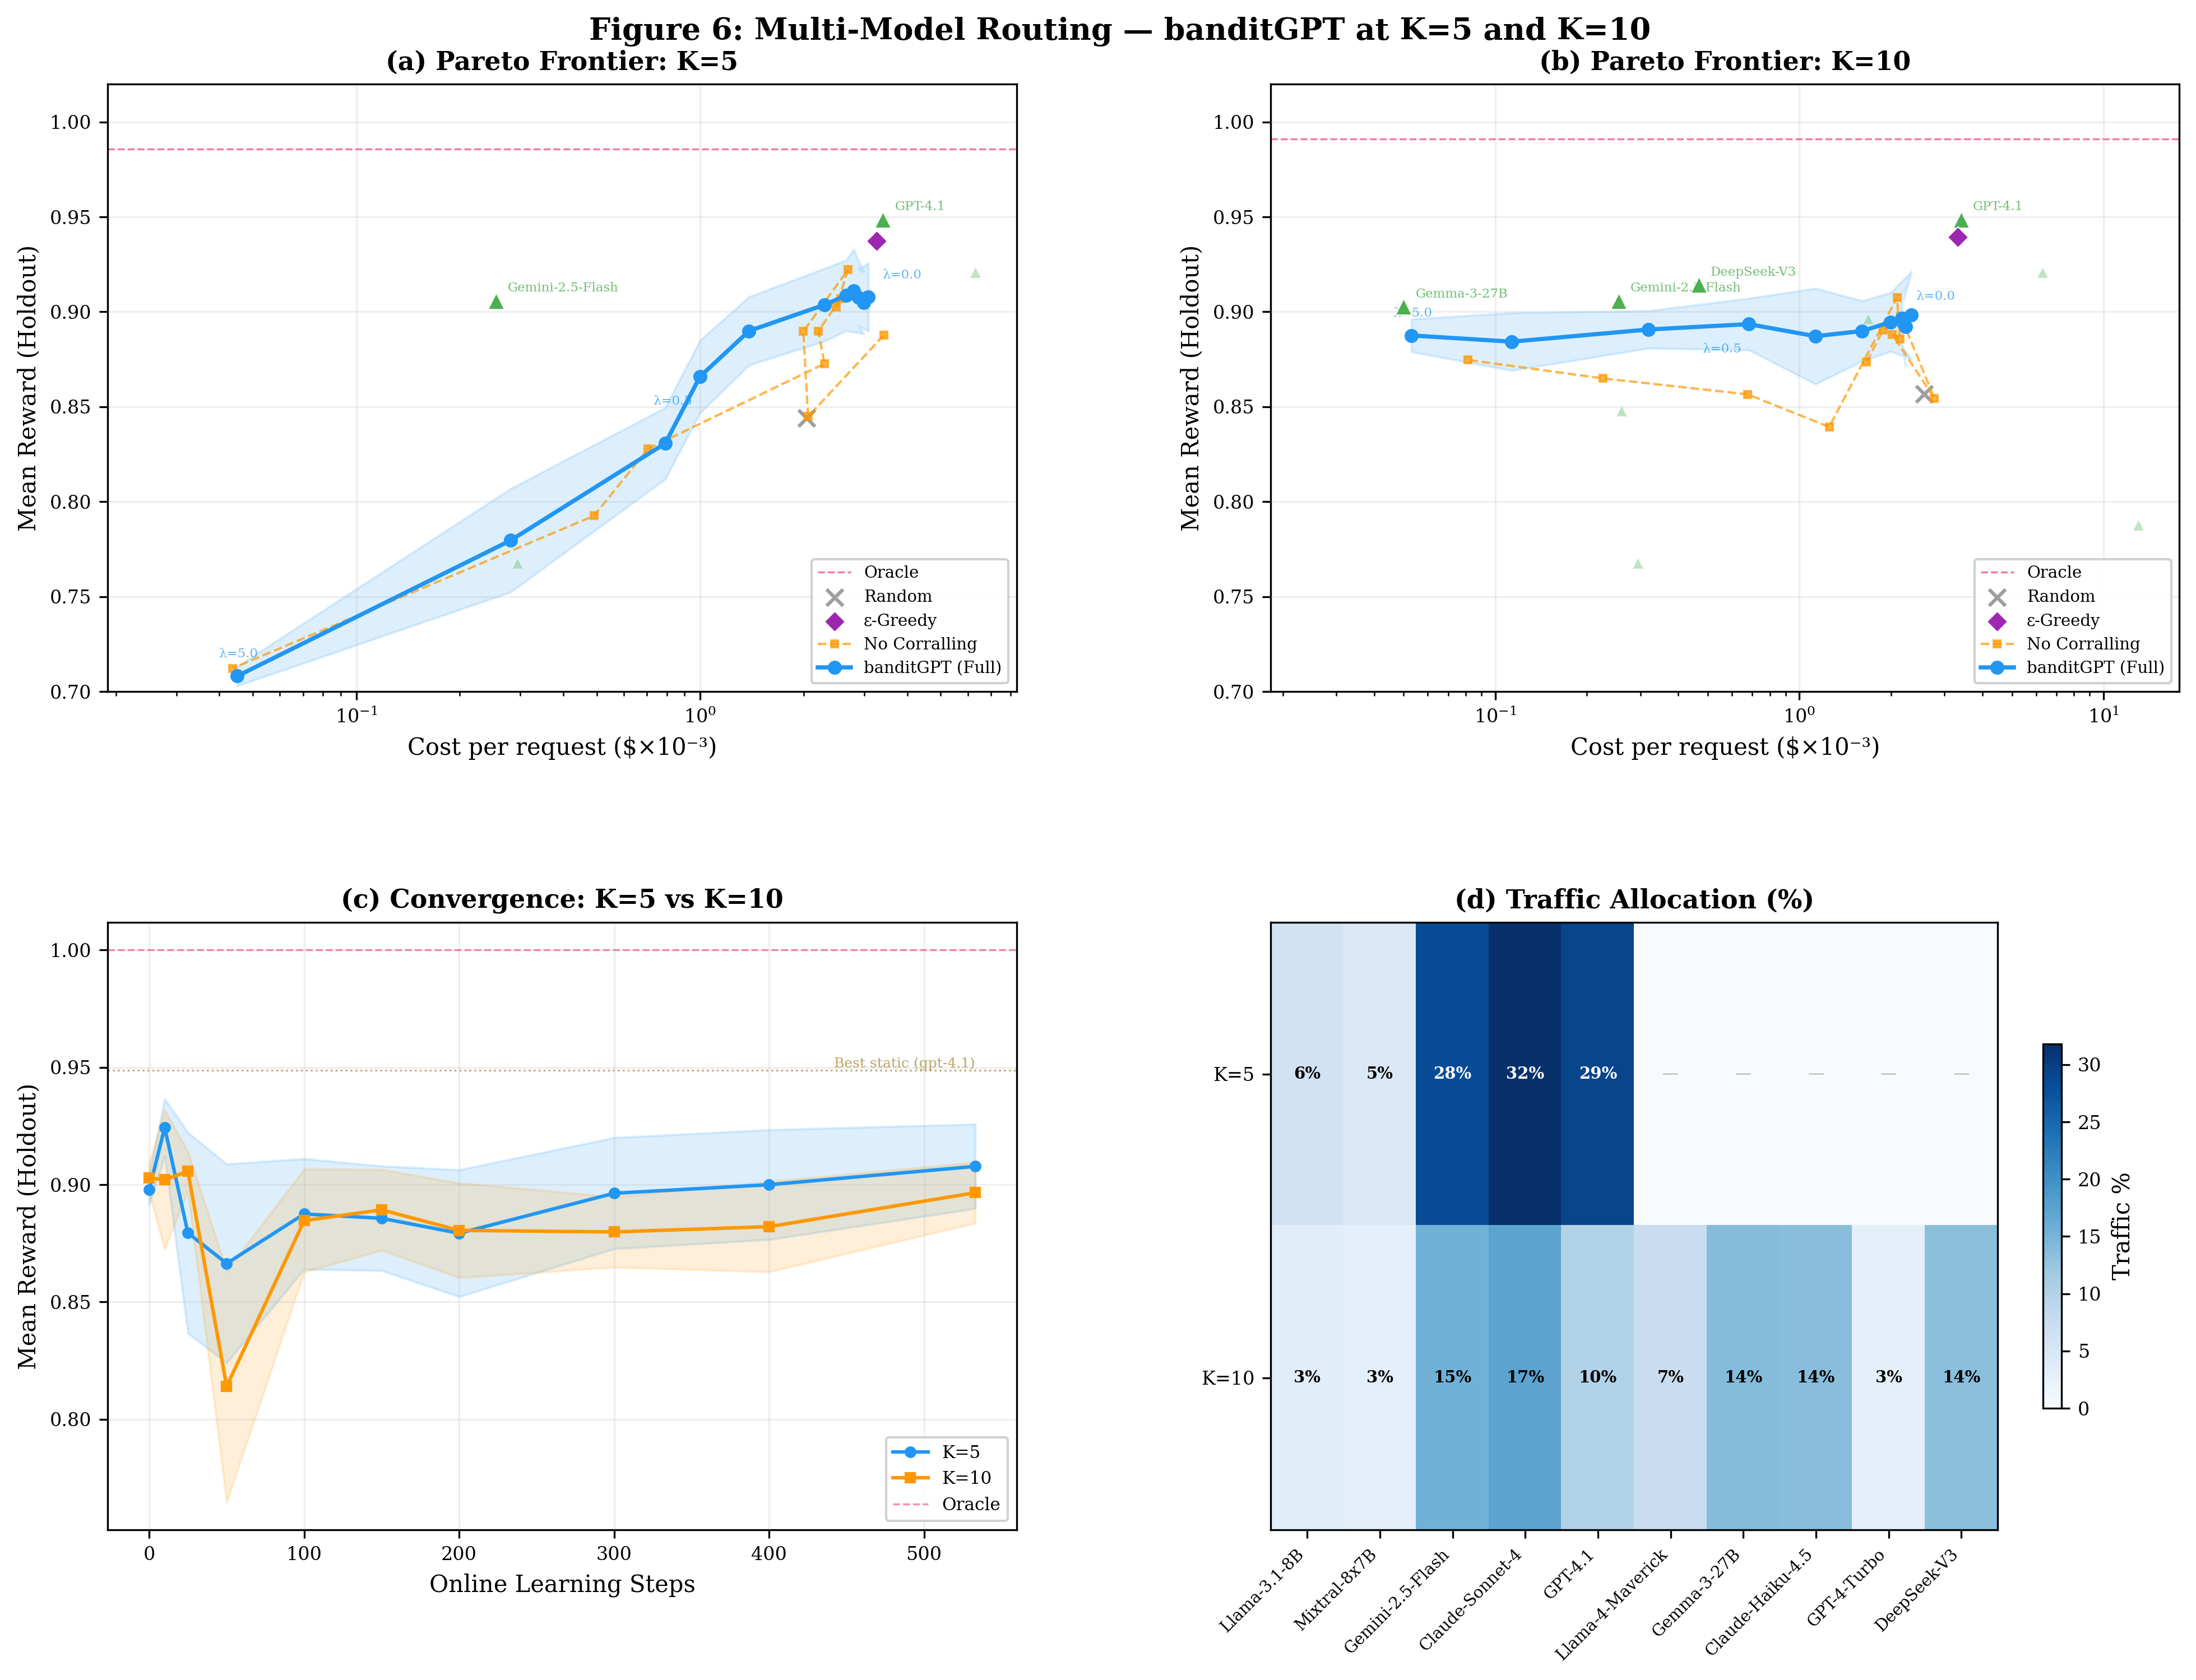
\includegraphics[width=0.95\textwidth]{../experiments/06_figure/results/figure6_multimodel_pareto.png}
\caption{\textbf{Multi-model routing at $K{=}5$ and $K{=}10$: cost--quality Pareto frontiers, convergence, and traffic allocation.} Reward is mean judge agreement across a 3--4 member LLM panel (continuous in $[0,1]$).
\textbf{(a,b)}~Pareto frontiers sweeping cost penalty $\lambda \in [0, 5]$ ($n{=}20$ seeds per point; log-scaled cost axis). Labelled green triangles mark Pareto-efficient static baselines; faded triangles show dominated models. The blue curve traces banditGPT's operating envelope. At peak quality ($\lambda{=}0.02$), banditGPT achieves 0.911 (K{=}5) and 0.898 (K{=}10). At $\lambda{=}5$ (cost-minimising), it routes nearly all traffic to the cheapest model while maintaining 0.708 (K{=}5) and 0.888 (K{=}10) quality. The orange dashed line (no Corralling) shows the ablated system without the meta-learner.
\textbf{(c)}~Convergence from warmup priors: both portfolios start at ${\sim}0.90$ reward (step~0, no online learning), demonstrating that the 43-model warmup priors provide effective cold-start quality across portfolio sizes. K{=}5 improves to 0.911 by step 533; K{=}10 remains stable at ${\sim}0.88{-}0.90$.
\textbf{(d)}~Traffic allocation on the holdout set ($\lambda{=}0$). At K{=}5, the router concentrates on three high-quality models (Claude-Sonnet: 32\%, GPT-4.1: 29\%, Gemini-Flash: 28\%) while using cheaper models sparingly (${\leq}6\%$). At K{=}10, traffic distributes across all models (3--17\% each), reflecting contextual per-prompt routing rather than static model selection.
Evaluation protocol: 533 online-learning prompts (three-way split, disjoint from prior training), frozen holdout of 750 prompts (identical to Section~\ref{sec:pareto}).}
\label{fig:multimodel_pareto}
\end{figure*}


\begin{figure*}[t]
\centering
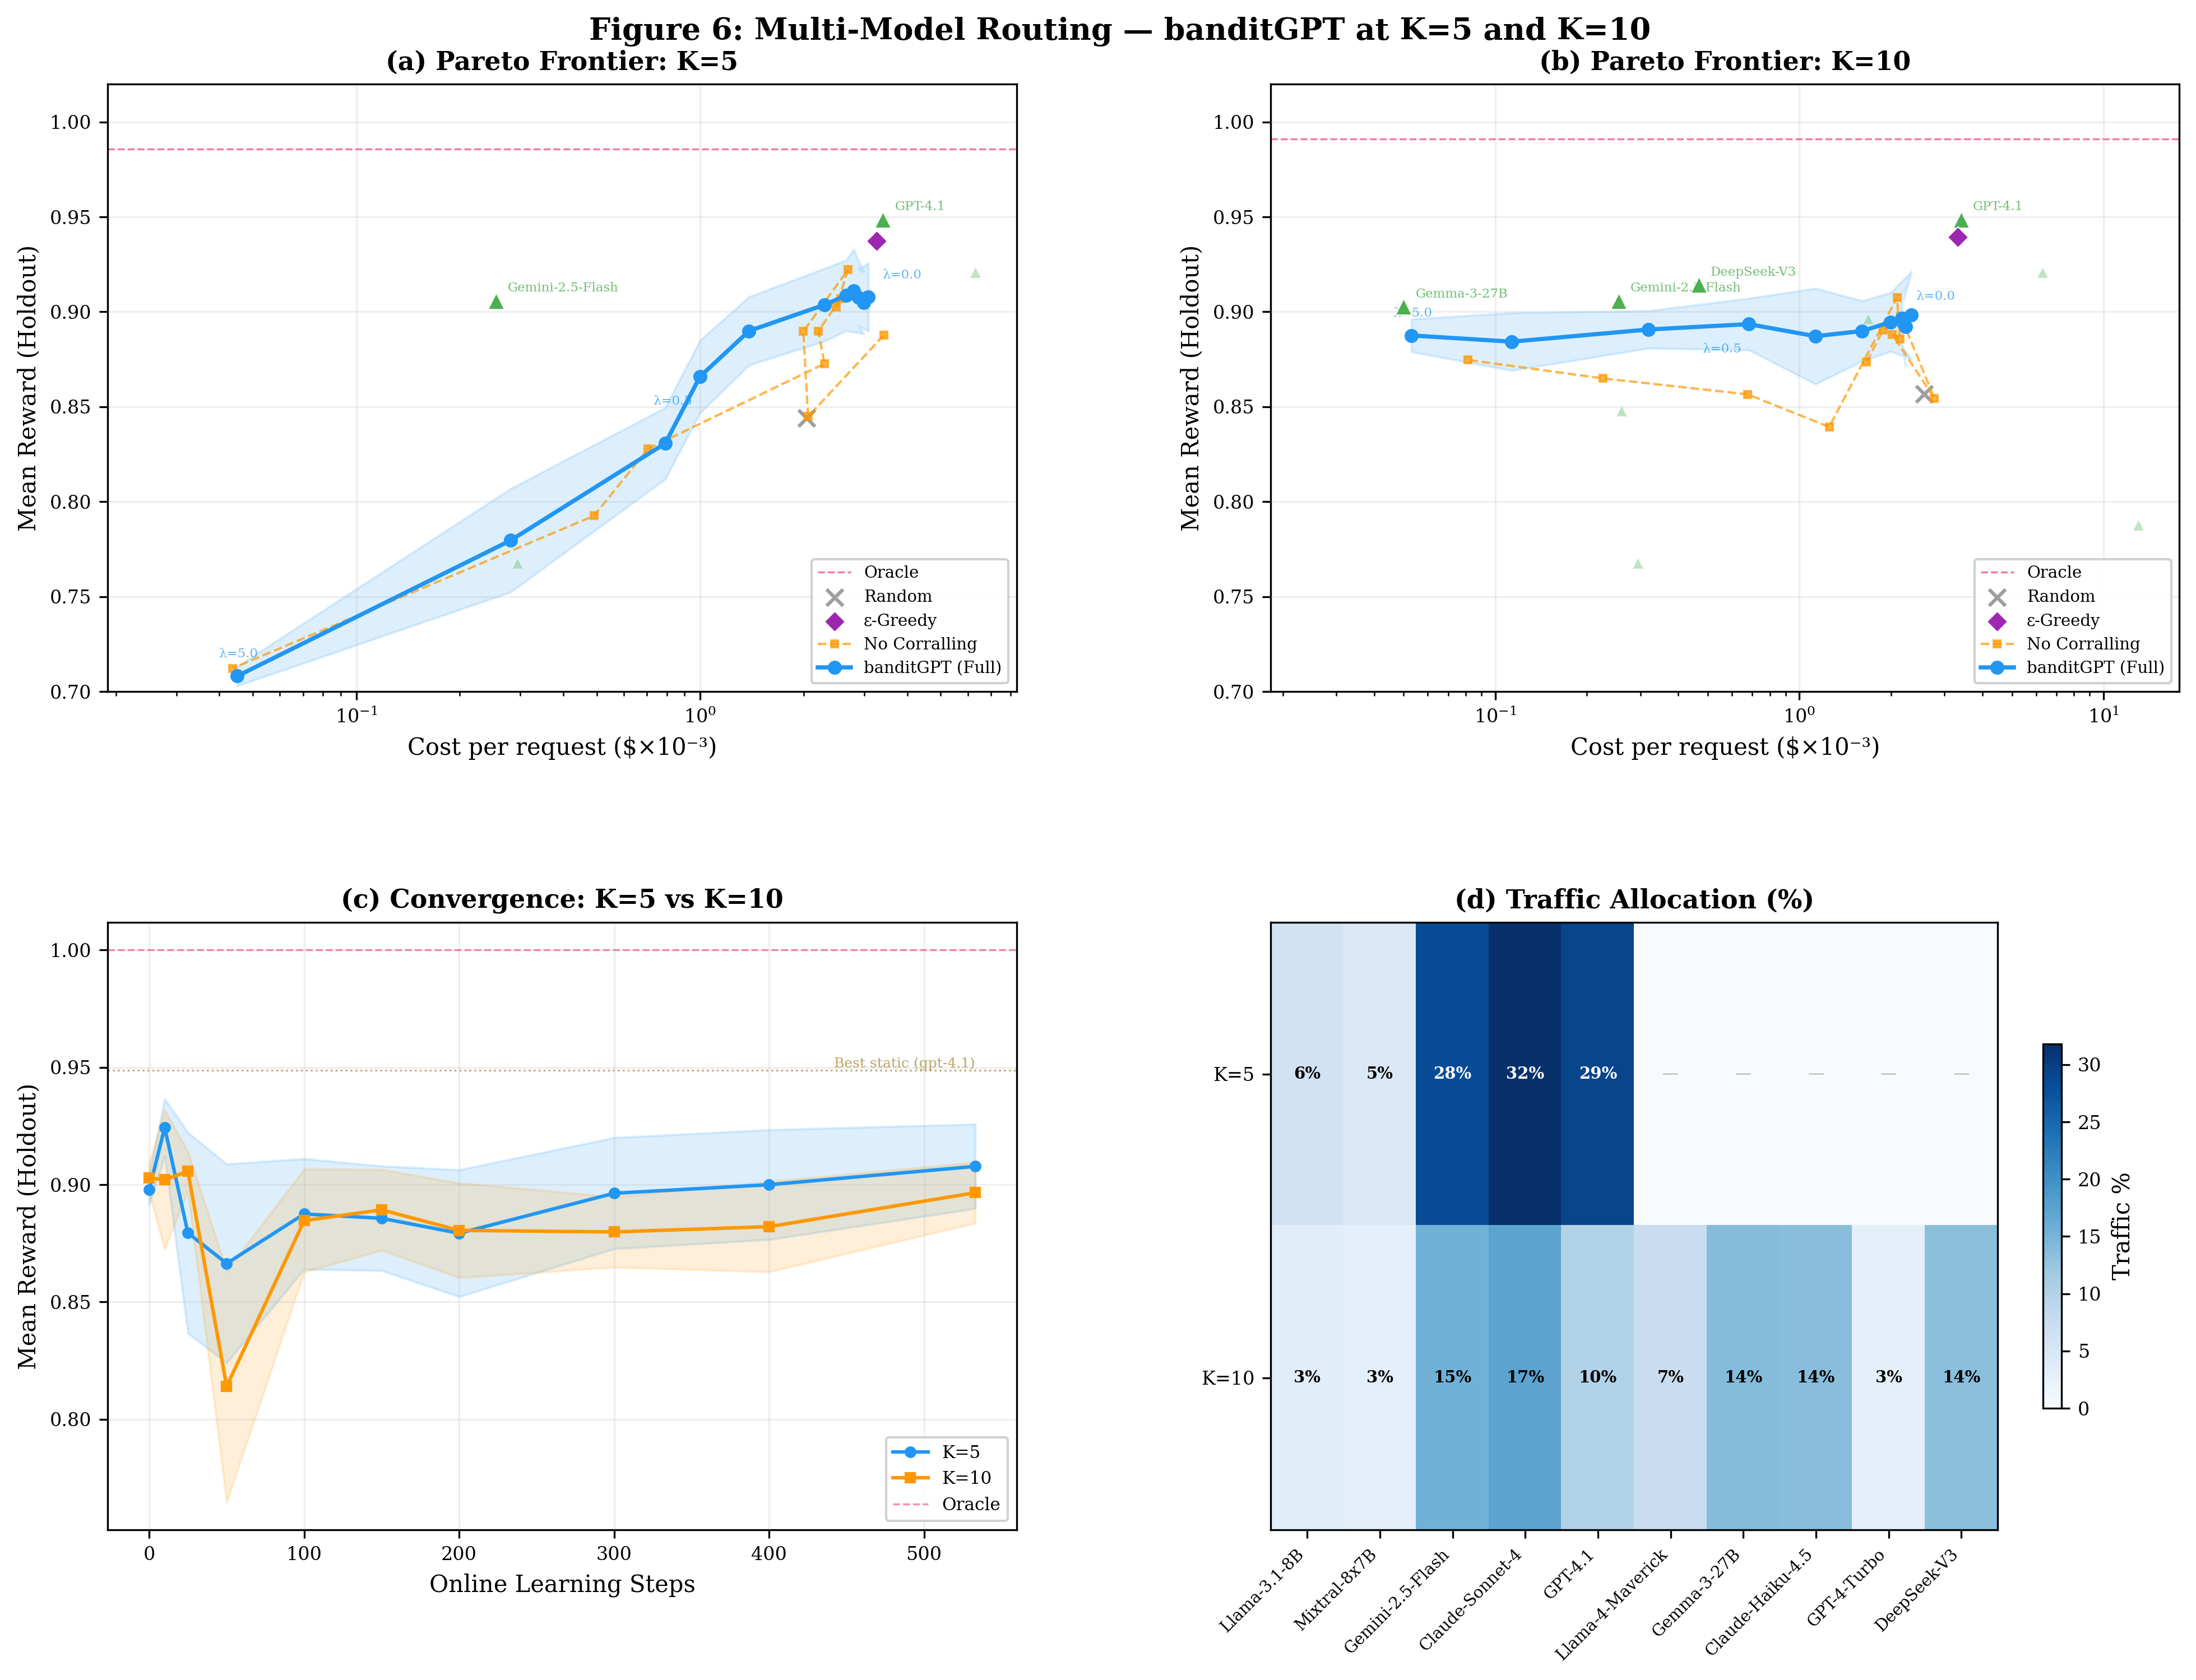
\includegraphics[width=0.95\textwidth]{../experiments/06_figure/results/figure6_multimodel_pareto.png}
\caption{\textbf{Multi-model routing at $K{=}5$ and $K{=}10$: cost--quality Pareto frontiers, convergence, and traffic allocation.} Reward is mean judge agreement across a 3--4 member LLM panel (continuous in $[0,1]$).
\textbf{(a,b)}~Pareto frontiers sweeping cost penalty $\lambda \in [0, 5]$ ($n{=}20$ seeds per point; log-scaled cost axis). Labelled green triangles mark Pareto-efficient static baselines; faded triangles show dominated models. The blue curve traces banditGPT's operating envelope. At peak quality ($\lambda{=}0.02$), banditGPT achieves 0.911 (K{=}5) and 0.898 (K{=}10). At $\lambda{=}5$ (cost-minimising), it routes nearly all traffic to the cheapest model while maintaining 0.708 (K{=}5) and 0.888 (K{=}10) quality. The orange dashed line (no Corralling) shows the ablated system without the meta-learner.
\textbf{(c)}~Convergence from warmup priors: both portfolios start at ${\sim}0.90$ reward (step~0, no online learning), demonstrating that the 43-model warmup priors provide effective cold-start quality across portfolio sizes. K{=}5 improves to 0.911 by step 533; K{=}10 remains stable at ${\sim}0.88{-}0.90$.
\textbf{(d)}~Traffic allocation on the holdout set ($\lambda{=}0$). At K{=}5, the router concentrates on three high-quality models (Claude-Sonnet: 32\%, GPT-4.1: 29\%, Gemini-Flash: 28\%) while using cheaper models sparingly (${\leq}6\%$). At K{=}10, traffic distributes across all models (3--17\% each), reflecting contextual per-prompt routing rather than static model selection.
Evaluation protocol: 533 online-learning prompts (three-way split, disjoint from prior training), frozen holdout of 750 prompts (identical to Section~\ref{sec:pareto}).}
\label{fig:multimodel_pareto}
\end{figure*}


\begin{figure*}[t]
\centering
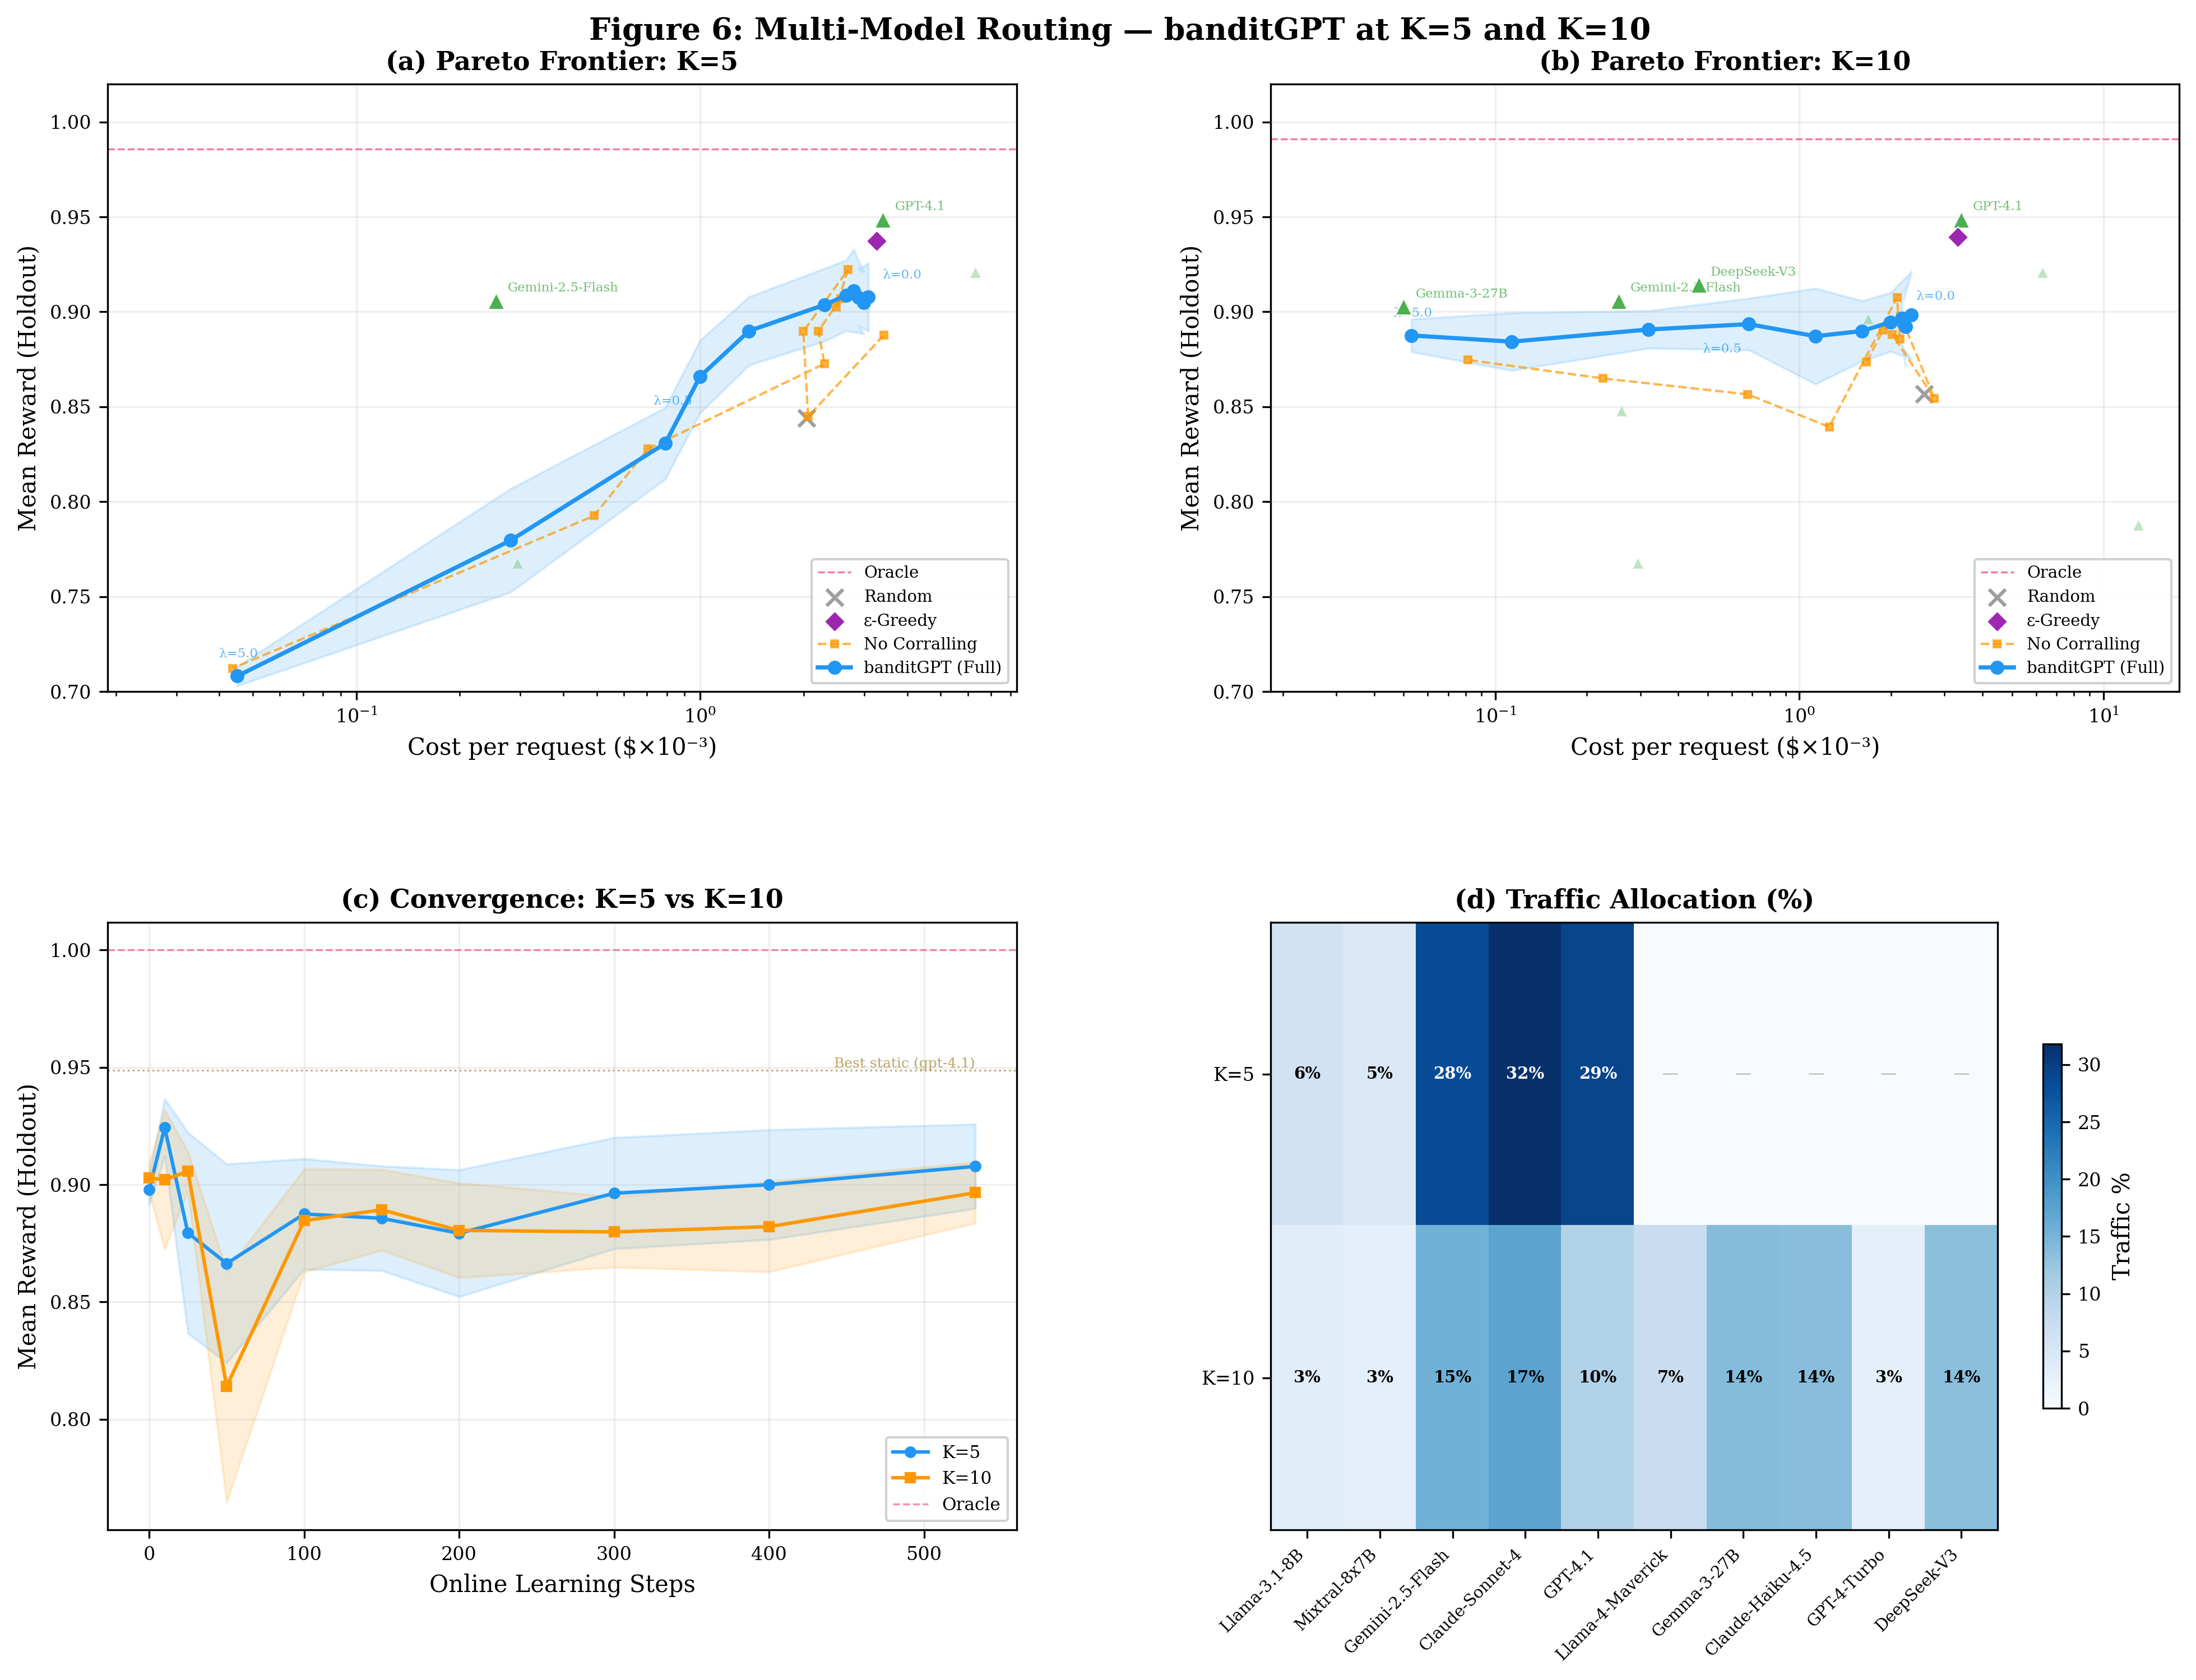
\includegraphics[width=0.95\textwidth]{../experiments/06_figure/results/figure6_multimodel_pareto.png}
\caption{\textbf{Multi-model routing at $K{=}5$ and $K{=}10$: cost--quality Pareto frontiers, convergence, and traffic allocation.} Reward is mean judge agreement across a 3--4 member LLM panel (continuous in $[0,1]$).
\textbf{(a,b)}~Pareto frontiers sweeping cost penalty $\lambda \in [0, 5]$ ($n{=}20$ seeds per point; log-scaled cost axis). Labelled green triangles mark Pareto-efficient static baselines; faded triangles show dominated models. The blue curve traces banditGPT's operating envelope. At peak quality ($\lambda{=}0.02$), banditGPT achieves 0.911 (K{=}5) and 0.898 (K{=}10). At $\lambda{=}5$ (cost-minimising), it routes nearly all traffic to the cheapest model while maintaining 0.708 (K{=}5) and 0.888 (K{=}10) quality. The orange dashed line (no Corralling) shows the ablated system without the meta-learner.
\textbf{(c)}~Convergence from warmup priors: both portfolios start at ${\sim}0.90$ reward (step~0, no online learning), demonstrating that the 43-model warmup priors provide effective cold-start quality across portfolio sizes. K{=}5 improves to 0.911 by step 533; K{=}10 remains stable at ${\sim}0.88{-}0.90$.
\textbf{(d)}~Traffic allocation on the holdout set ($\lambda{=}0$). At K{=}5, the router concentrates on three high-quality models (Claude-Sonnet: 32\%, GPT-4.1: 29\%, Gemini-Flash: 28\%) while using cheaper models sparingly (${\leq}6\%$). At K{=}10, traffic distributes across all models (3--17\% each), reflecting contextual per-prompt routing rather than static model selection.
Evaluation protocol: 533 online-learning prompts (three-way split, disjoint from prior training), frozen holdout of 750 prompts (identical to Section~\ref{sec:pareto}).}
\label{fig:multimodel_pareto}
\end{figure*}
